\section{Resultados}

\subsection{Métricas de calidad}

\begin{frame}{Resultados}{Métricas de calidad}

\begin{itemize}
    \justifying
    \item La \textbf{IoU} es una medida basada en el índice Jaccard que evalúa la superposición entre dos cuadros delimitadores.
\end{itemize}

    \begin{figure}[ht]
    \centering
    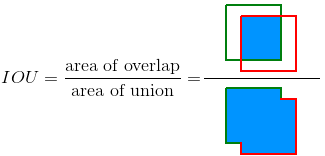
\includegraphics[width=0.4\textwidth]{Images/resultados/metricas/iou.png}
    \caption{\label{fig:iou}Área de superposición IoU entre los cuadros delimitadores}
    \end{figure}
    
\begin{itemize}
    \justifying
    \item True Positive (\textbf{TP}), True Negative (\textbf{TN}), False Positive (\textbf{FP}) y False Negative (\textbf{FN}).
    \item La \textbf{precisión} es la capacidad de un modelo para identificar solo los objetos relevantes.
\end{itemize}

\end{frame}

%%%%%%%%%%%%%%%%%%%%%%%%%%%%%%%%%%%%%%%%%%%%%%%%%%%%%%%%%%%%%%%%%

\begin{frame}{Resultados}{Métricas de calidad}

\begin{itemize}
    \justifying
    \setlength\itemsep{1em}
    \item El \textbf{Recall} es la capacidad de un modelo para encontrar todos los casos relevantes (todos los cuadros delimitadores de ground truth).
    \item El \textbf{F-Score} se trata de una medida estadística de precisión muy utilizada en las pruebas test de algoritmos.
    \item La precisión media (\textbf{AP}) es el valor medio de 11 puntos en la curva \textbf{P-R} para cada posible umbral (cada probabilidad de detección) para la misma clase (Precisión-Recall). Por otro lado, el \textbf{mAP} es la media de los \textbf{AP} de todas las categorías de objetos.
\end{itemize}

\end{frame}

%%%%%%%%%%%%%%%%%%%%%%%%%%%%%%%%%%%%%%%%%%%%%%%%%%%%%%%%%%%%%%%%%
\subsection{Bases de datos}

\begin{frame}{Resultados}{Bases de datos}

\begin{itemize}
    \justifying
    \item Resolución 768x576 a 25 fps.
    \item Cámaras 1 y 3: Canon MV-1 1xCCD w/progressive scan.
    \item Cámaras 2 y 4: Sony DCR-PC1000E 3xCMOS.
    \item Secuencias que contienen tres tipos de escenarios con una complejidad ascendente: personas merodeando, robo de equipaje y equipaje desatendido/abandonado.
\end{itemize}

\vspace{0.1cm}

\begin{figure}[ht]
  \centering
  \begin{subfigure}[b]{0.28\textwidth}
    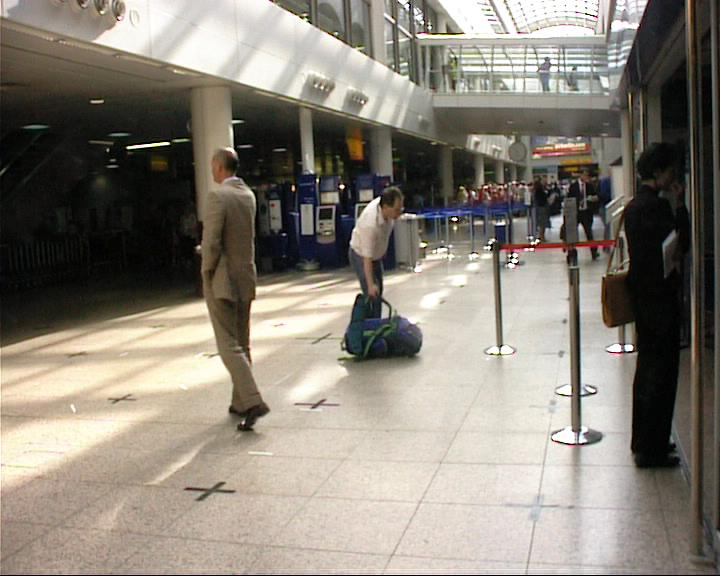
\includegraphics[width=\textwidth]{Images/resultados/datasets/pets2007_1.jpg}
    \caption{}
    \label{fig:pets2007_1}
  \end{subfigure}
  \qquad
  \begin{subfigure}[b]{0.28\textwidth}
    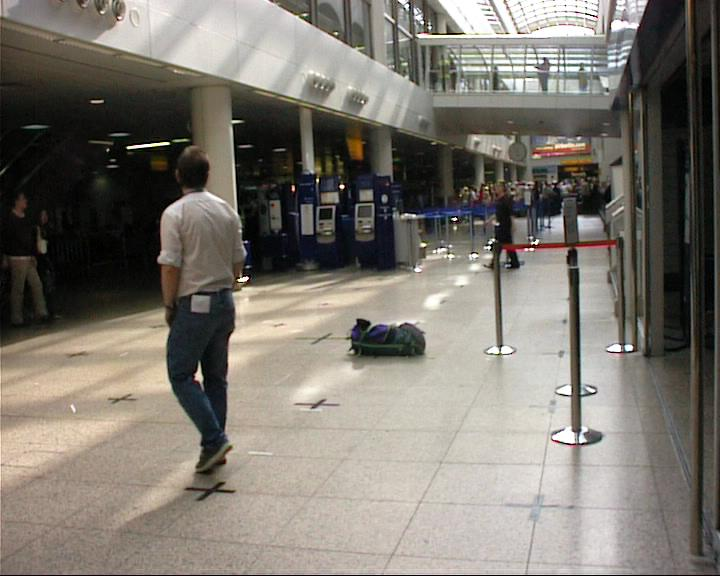
\includegraphics[width=\textwidth]{Images/resultados/datasets/pets2007_2.jpg}
    \caption{}
    \label{fig:pets2007_2}
  \end{subfigure}
  \caption{Imágenes extraídas del dataset PETS2007}
  \label{fig:pets2007}
\end{figure}

\end{frame}

%%%%%%%%%%%%%%%%%%%%%%%%%%%%%%%%%%%%%%%%%%%%%%%%%%%%%%%%%%%%%%%%%

\begin{frame}{Resultados}{Bases de datos}

\begin{itemize}
    \justifying
    \item Resolución 1920x1080 a 60 fps.
    \item Cámara GoPro HERO4.
    \item Contiene 8 secuencias en 2 escenarios donde tienen lugar eventos como abandono de maletas, mochilas y bolsas de mano.
\end{itemize}

\vspace{0.1cm}

\begin{figure}[ht]
  \centering
  \begin{subfigure}[b]{0.4\textwidth}
    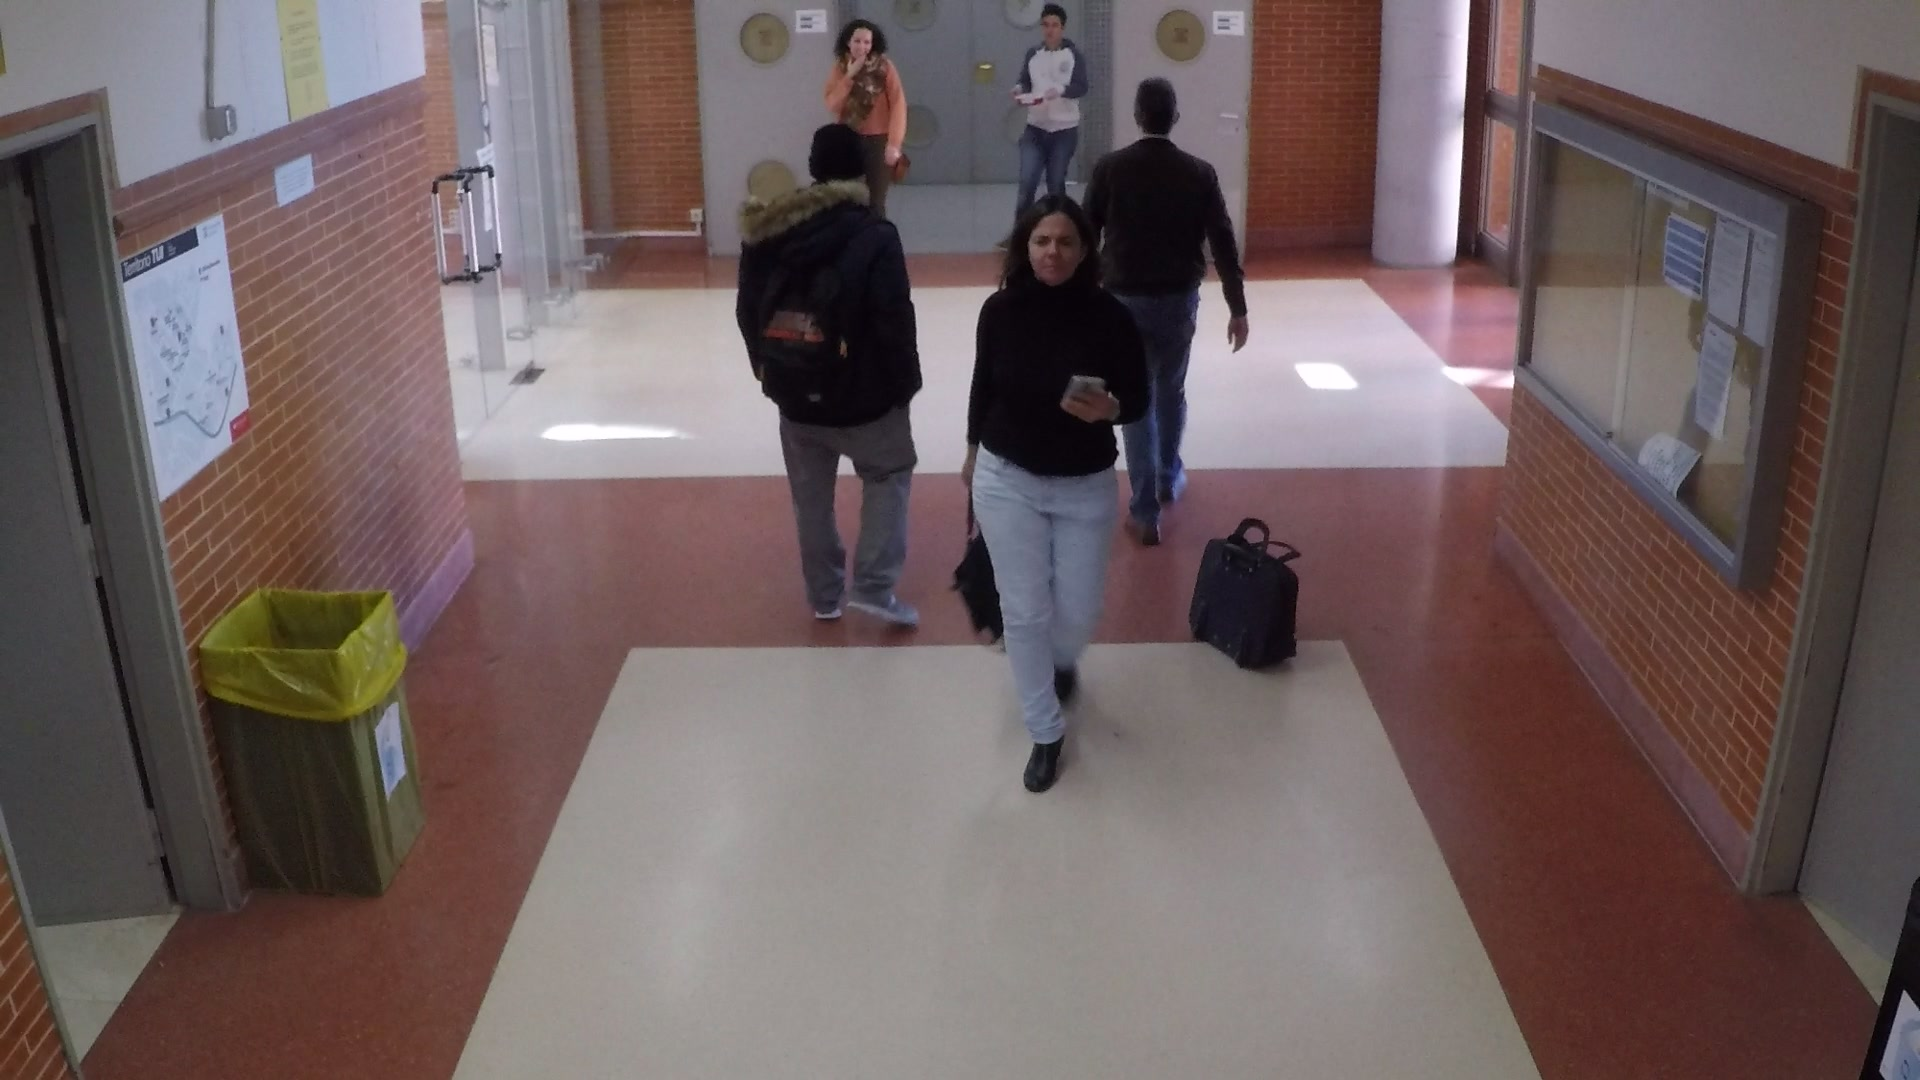
\includegraphics[width=\textwidth]{Images/resultados/datasets/GBA_3.jpg}
    \caption{}
    \label{fig:GBA_3}
  \end{subfigure}
  \qquad
  \begin{subfigure}[b]{0.4\textwidth}
    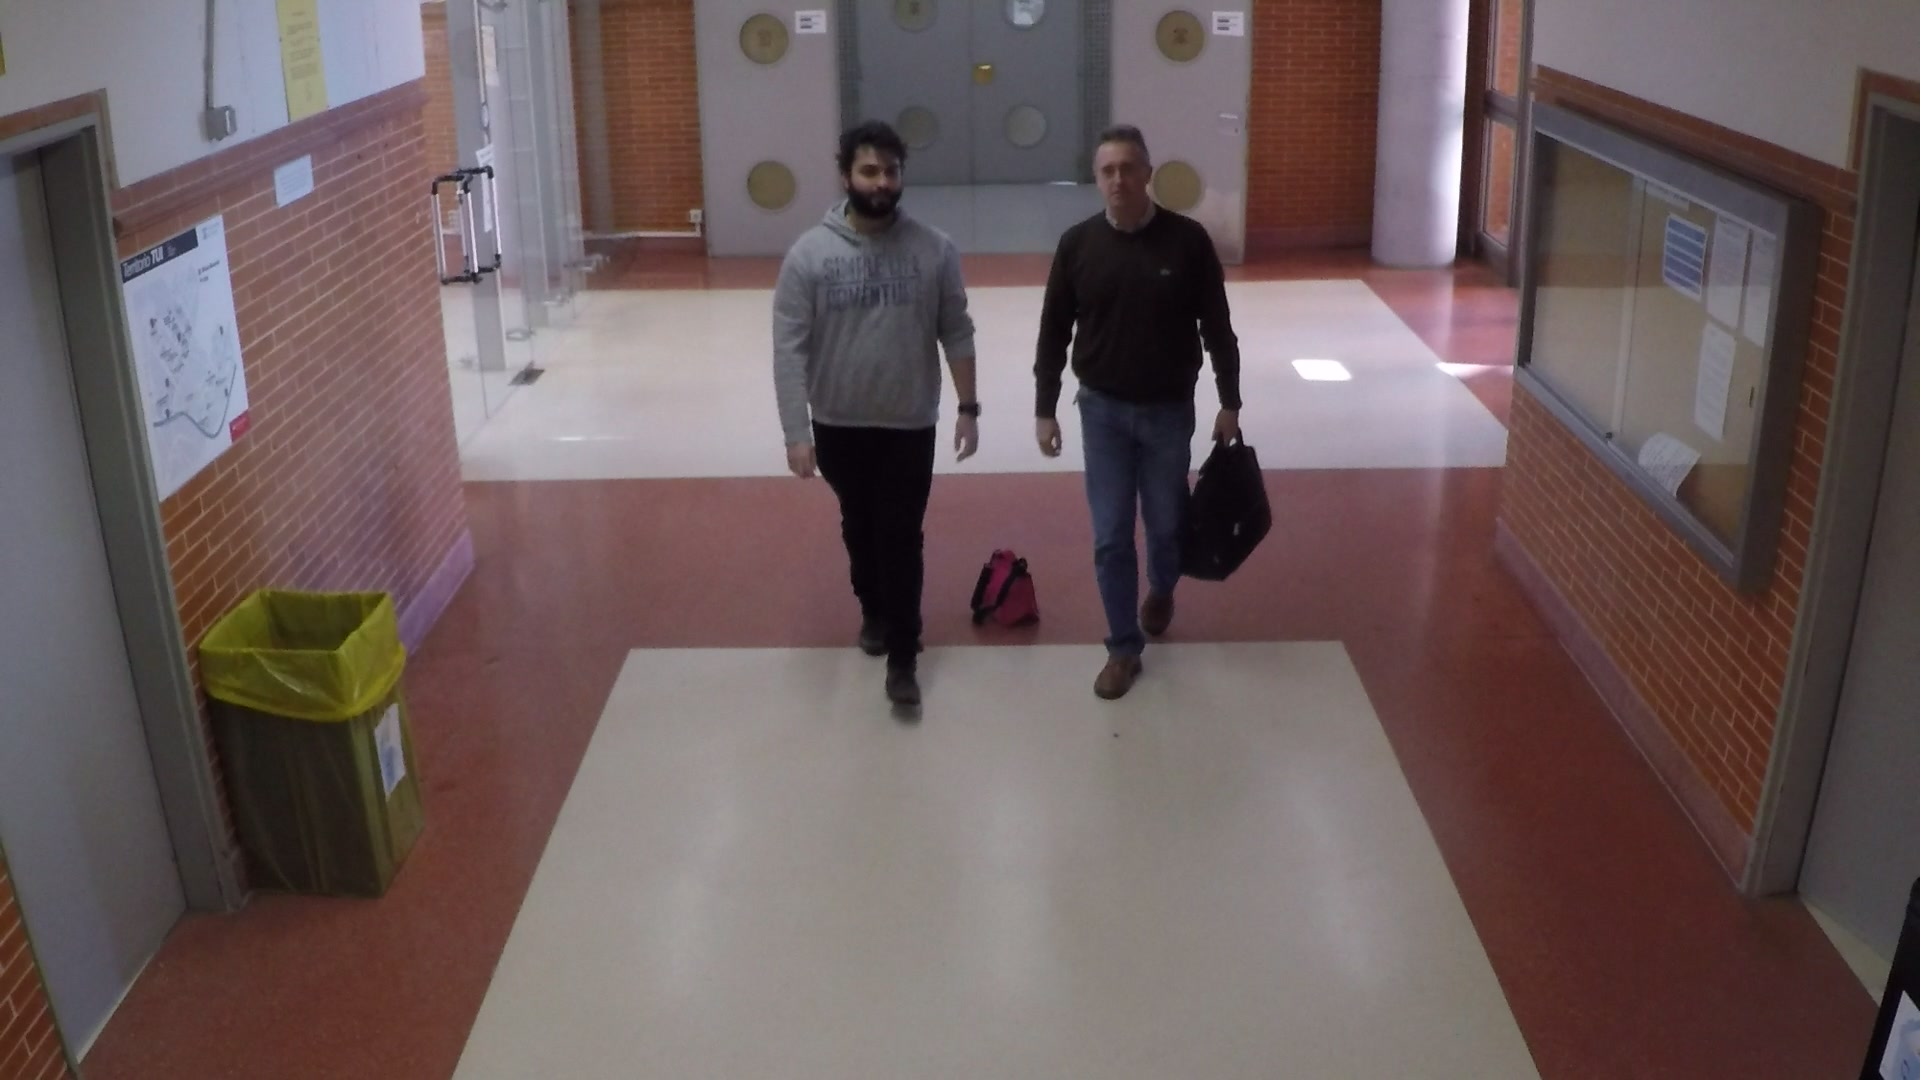
\includegraphics[width=\textwidth]{Images/resultados/datasets/GBA_4.jpg}
    \caption{}
    \label{fig:GBA_4}
  \end{subfigure}
  \caption{Imágenes extraídas del dataset GBA2018}
  \label{fig:GBA2018}
\end{figure}
    
\end{frame}

%%%%%%%%%%%%%%%%%%%%%%%%%%%%%%%%%%%%%%%%%%%%%%%%%%%%%%%%%%%%%%%%%

\begin{frame}{Resultados}{Bases de datos}

\begin{itemize}
    \justifying
    \item Resolución 720x576 a 25 fps.
    \item Modelo de la cámara no especificado.
    \item Subconjunto de datos del dataset AVSS 2007 creado para el i-LIDS bag and vehicle detection challenge.
    \item La región de interés está dividida en tres zonas: cercana, media y lejana.
\end{itemize}

\vspace{0.1cm}

\begin{figure}[ht]
  \centering
  \begin{subfigure}[b]{0.28\textwidth}
    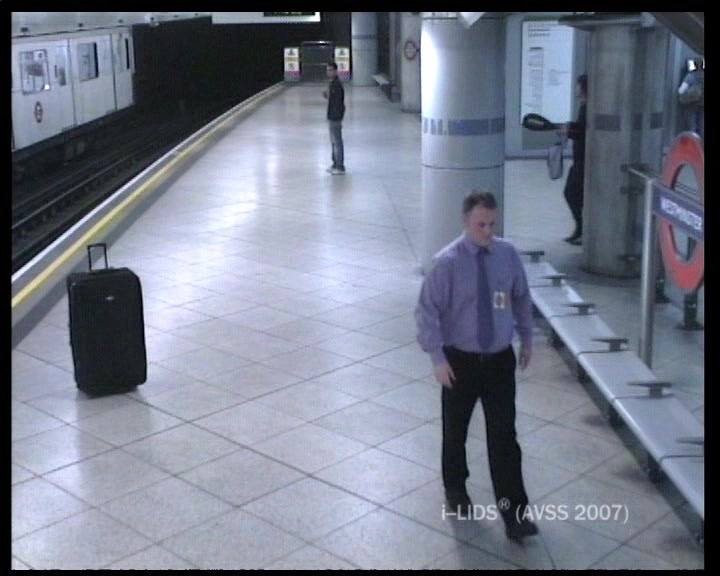
\includegraphics[width=\textwidth]{Images/resultados/datasets/AVSSAB_1.jpg}
    \caption{}
    \label{fig:AVSSAB_1}
  \end{subfigure}
  \qquad
  \begin{subfigure}[b]{0.28\textwidth}
    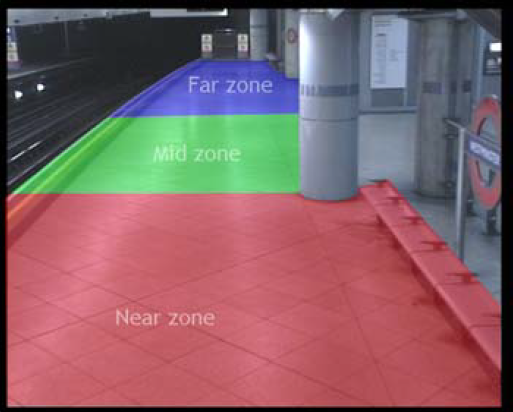
\includegraphics[width=\textwidth]{Images/resultados/datasets/avssab2007-zones.png}
    \caption{}
    \label{fig:AVSSAB_2}
  \end{subfigure}
  \caption{Imágenes extraídas del dataset AVSSAB2007}
  \label{fig:AVSSAB2007}
\end{figure}
    
\end{frame}

%%%%%%%%%%%%%%%%%%%%%%%%%%%%%%%%%%%%%%%%%%%%%%%%%%%%%%%%%%%%%%%%%

\begin{frame}{Resultados}{Bases de datos}

\begin{itemize}
    \justifying
    \item Resoluciones de 720x480 a 30 fps y 640x480 a 30 fps.
    \item Modelo de la cámara no especificado.
    \item 11 secuencias etiquetadas con varios escenarios de aplicaciones reales.
    \item Escenas de aglomeraciones de personas que se encuentran en aeropuertos o estaciones de tren, iluminación variable de día y grabaciones nocturnas.
\end{itemize}

\vspace{0.1cm}

\begin{figure}[ht]
  \centering
  \begin{subfigure}[b]{0.3\textwidth}
    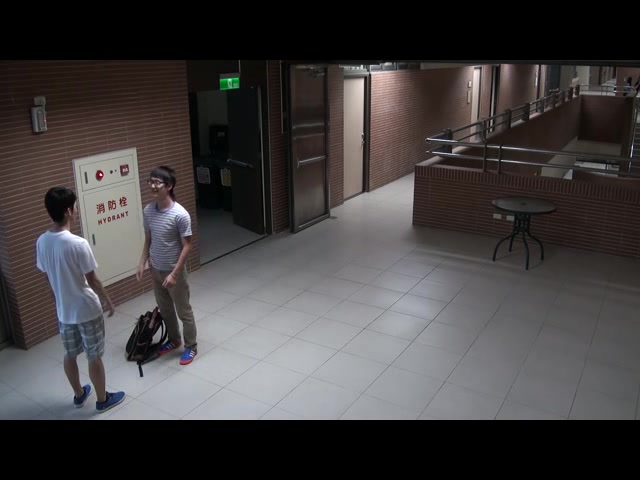
\includegraphics[width=\textwidth]{Images/resultados/datasets/aboda_1.jpg}
    \caption{}
    \label{fig:aboda_1}
  \end{subfigure}
  \qquad
  \begin{subfigure}[b]{0.3\textwidth}
    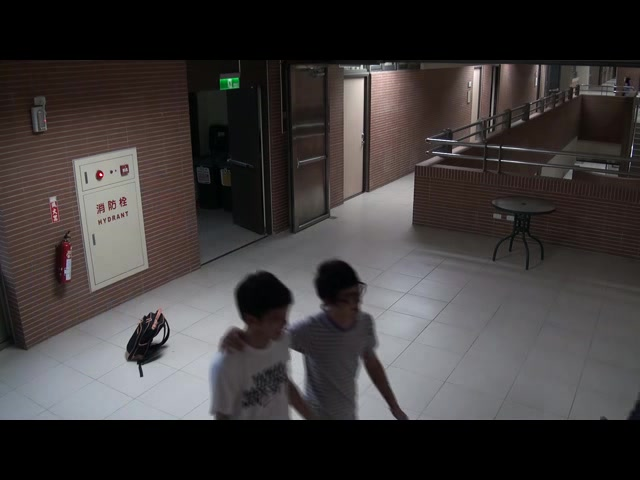
\includegraphics[width=\textwidth]{Images/resultados/datasets/aboda_2.jpg}
    \caption{}
    \label{fig:aboda_2}
  \end{subfigure}
  \caption{Imágenes extraídas del dataset ABODA}
  \label{fig:aboda}
\end{figure}
    
\end{frame}

%%%%%%%%%%%%%%%%%%%%%%%%%%%%%%%%%%%%%%%%%%%%%%%%%%%%%%%%%%%%%%%%%

\subsection{Resultados entrenamientos}

\begin{frame}{Resultados}{Resultados de los entrenamientos vs MS COCO}

\begin{table}[ht]
\centering
\label{tab:comparativa-metricas1}
\begin{tabular}{lccc}
\hline
\textbf{Dataset}                   & \textbf{TP}          & \textbf{FP}          & \textbf{FN}          \\ \hline
\textbf{MS COCO}                   & \textbf{22.730}      & \textbf{10.889}      & \textbf{13.027}      \\
OIDv4 test 1                       & 430                  & 527                  & 273                  \\
OIDv4 test 2                       & 6.600                & 7.366                & 5.226                \\ \hline
\end{tabular}
\caption{Comparativa métricas de calidad entre los test en OIDv4 y MS COCO [1]}
\end{table}

\begin{table}[ht]
\centering
\label{tab:comparativa-metricas2}
\begin{tabular}{cccccc}
\hline
\textbf{Dataset}             & \textbf{\begin{tabular}[c]{@{}c@{}}Precision\\ (\%)\end{tabular}} & \textbf{\begin{tabular}[c]{@{}c@{}}Recall\\ (\%)\end{tabular}} & \textbf{\begin{tabular}[c]{@{}c@{}}F-score\\ (\%)\end{tabular}} & \textbf{\begin{tabular}[c]{@{}c@{}}average IoU\\ (\%)\end{tabular}} & \textbf{\begin{tabular}[c]{@{}c@{}}mAP @ 0.5\\ (\%)\end{tabular}} \\ \hline
\textbf{MS COCO}             & \textbf{67,61}                                                    & \textbf{63,57}                                                 & \textbf{65,53}                                                  & \textbf{56,04}                                                      & \textbf{64,16}                                                    \\
OIDv4 test 1                 & 44,93                                                             & 61,17                                                          & 51,81                                                           & 34,13                                                               & 66,25                                                             \\
OIDv4 test 2                 & 47,26                                                             & 55,81                                                          & 51,18                                                           & 37,83                                                               & 60,97                                                             \\ \hline
\end{tabular}
\caption{Comparativa métricas de calidad entre los dos test en OIDv4 y MS COCO [2]}
\end{table}

\end{frame}

%%%%%%%%%%%%%%%%%%%%%%%%%%%%%%%%%%%%%%%%%%%%%%%%%%%%%%%%%%%%%%%%%

\subsection{Resultados detección, seguimiento y detección de objetos abandonados}

\begin{frame}{Resultados}{Resultados detección de personas y objetos}

\begin{itemize}
    \item blablabla
    \item blablabla
    \item blablabla
\end{itemize}

\begin{figure}[ht]
\centering
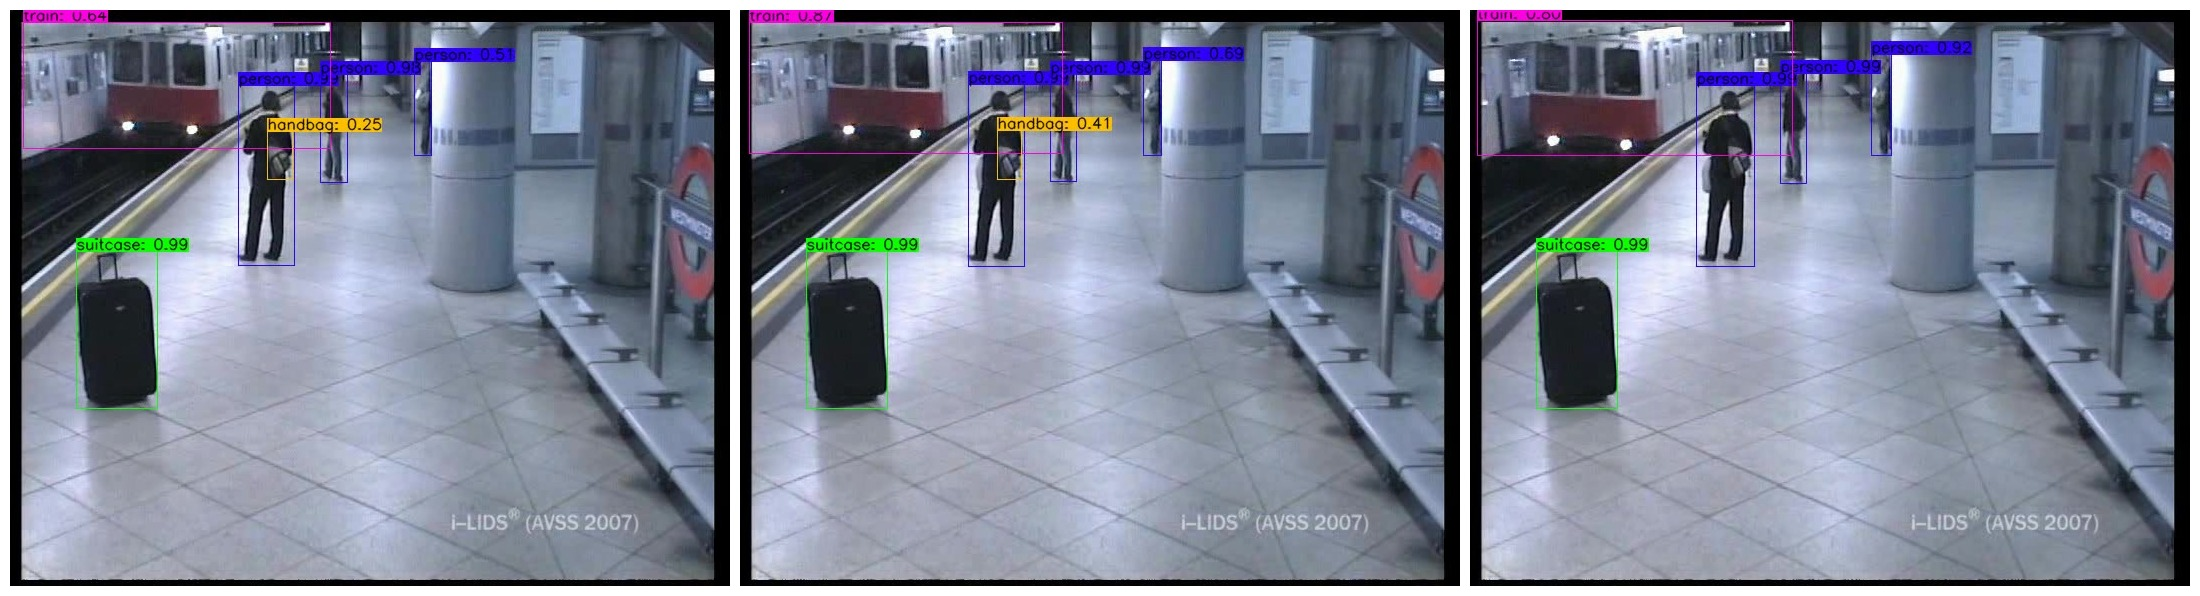
\includegraphics[width=1\textwidth]{Images/resultados/evaluacion-algoritmos/avss-easy-detection-example.jpg}
\caption{\label{fig:avss-easy-detection-example}Detección de personas y objetos en el dataset AVSSAB2007}
\end{figure}

\end{frame}

%%%%%%%%%%%%%%%%%%%%%%%%%%%%%%%%%%%%%%%%%%%%%%%%%%%%%%%%%%%%%%%%%

\begin{frame}{Resultados}{Resultados seguimiento de personas y objetos}

\begin{itemize}
    \item blablabla
    \item blablabla
    \item blablabla
\end{itemize}

\begin{figure}[ht]
\centering
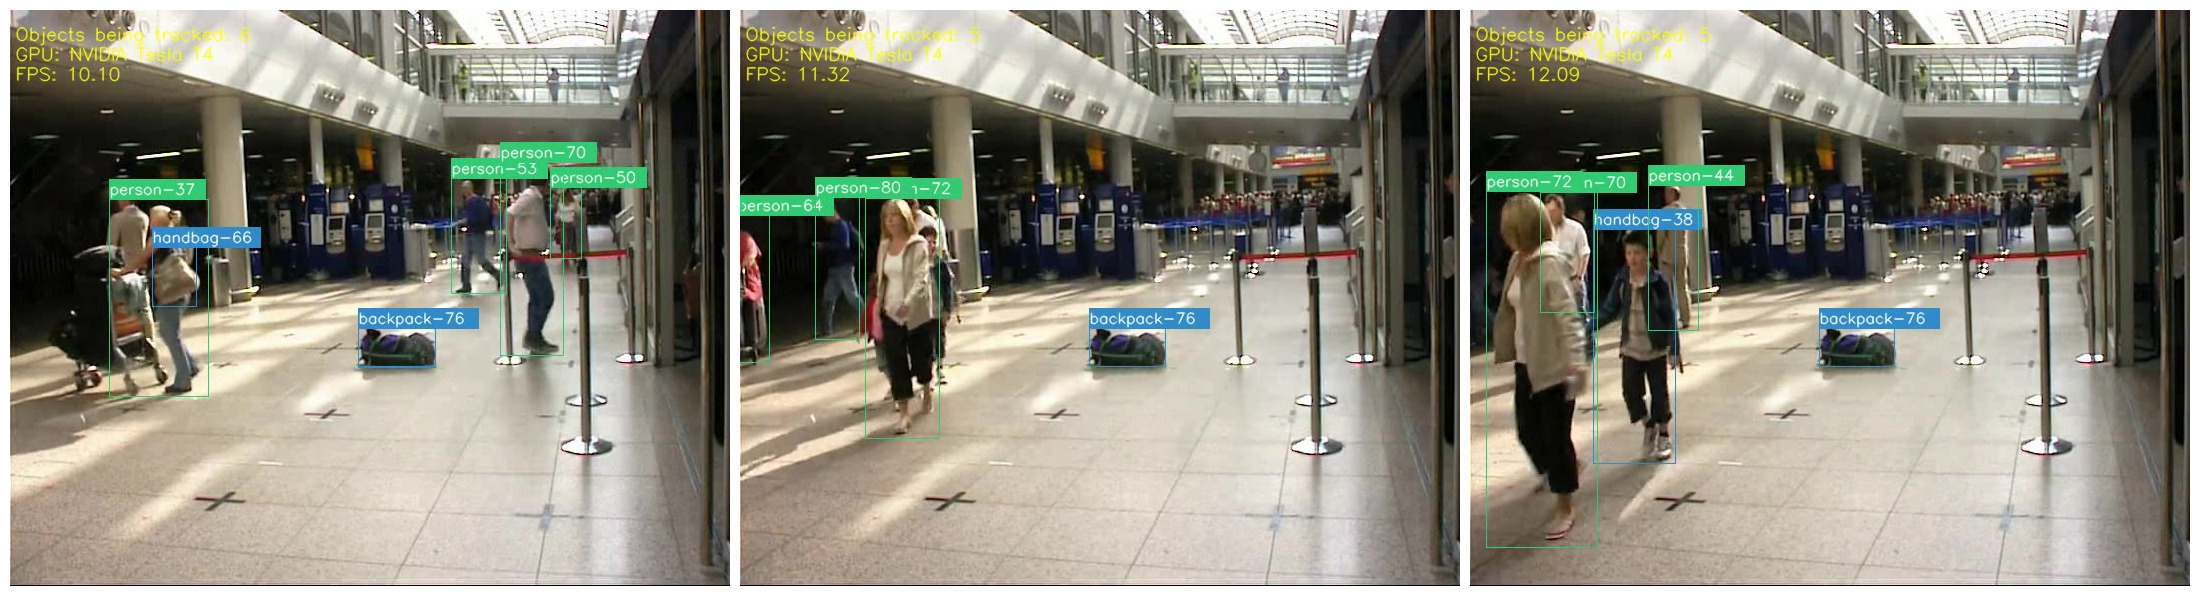
\includegraphics[width=1\textwidth]{Images/resultados/evaluacion-algoritmos/pets-tracking-result-example.jpg}
\caption{\label{fig:pets-tracking-result-example}Seguimiento de personas y objetos en el dataset PETS2007}
\end{figure}

\end{frame}

%%%%%%%%%%%%%%%%%%%%%%%%%%%%%%%%%%%%%%%%%%%%%%%%%%%%%%%%%%%%%%%%%

\begin{frame}{Resultados}{Resultados detección objetos abandonados}

\begin{figure}[ht]
\centering
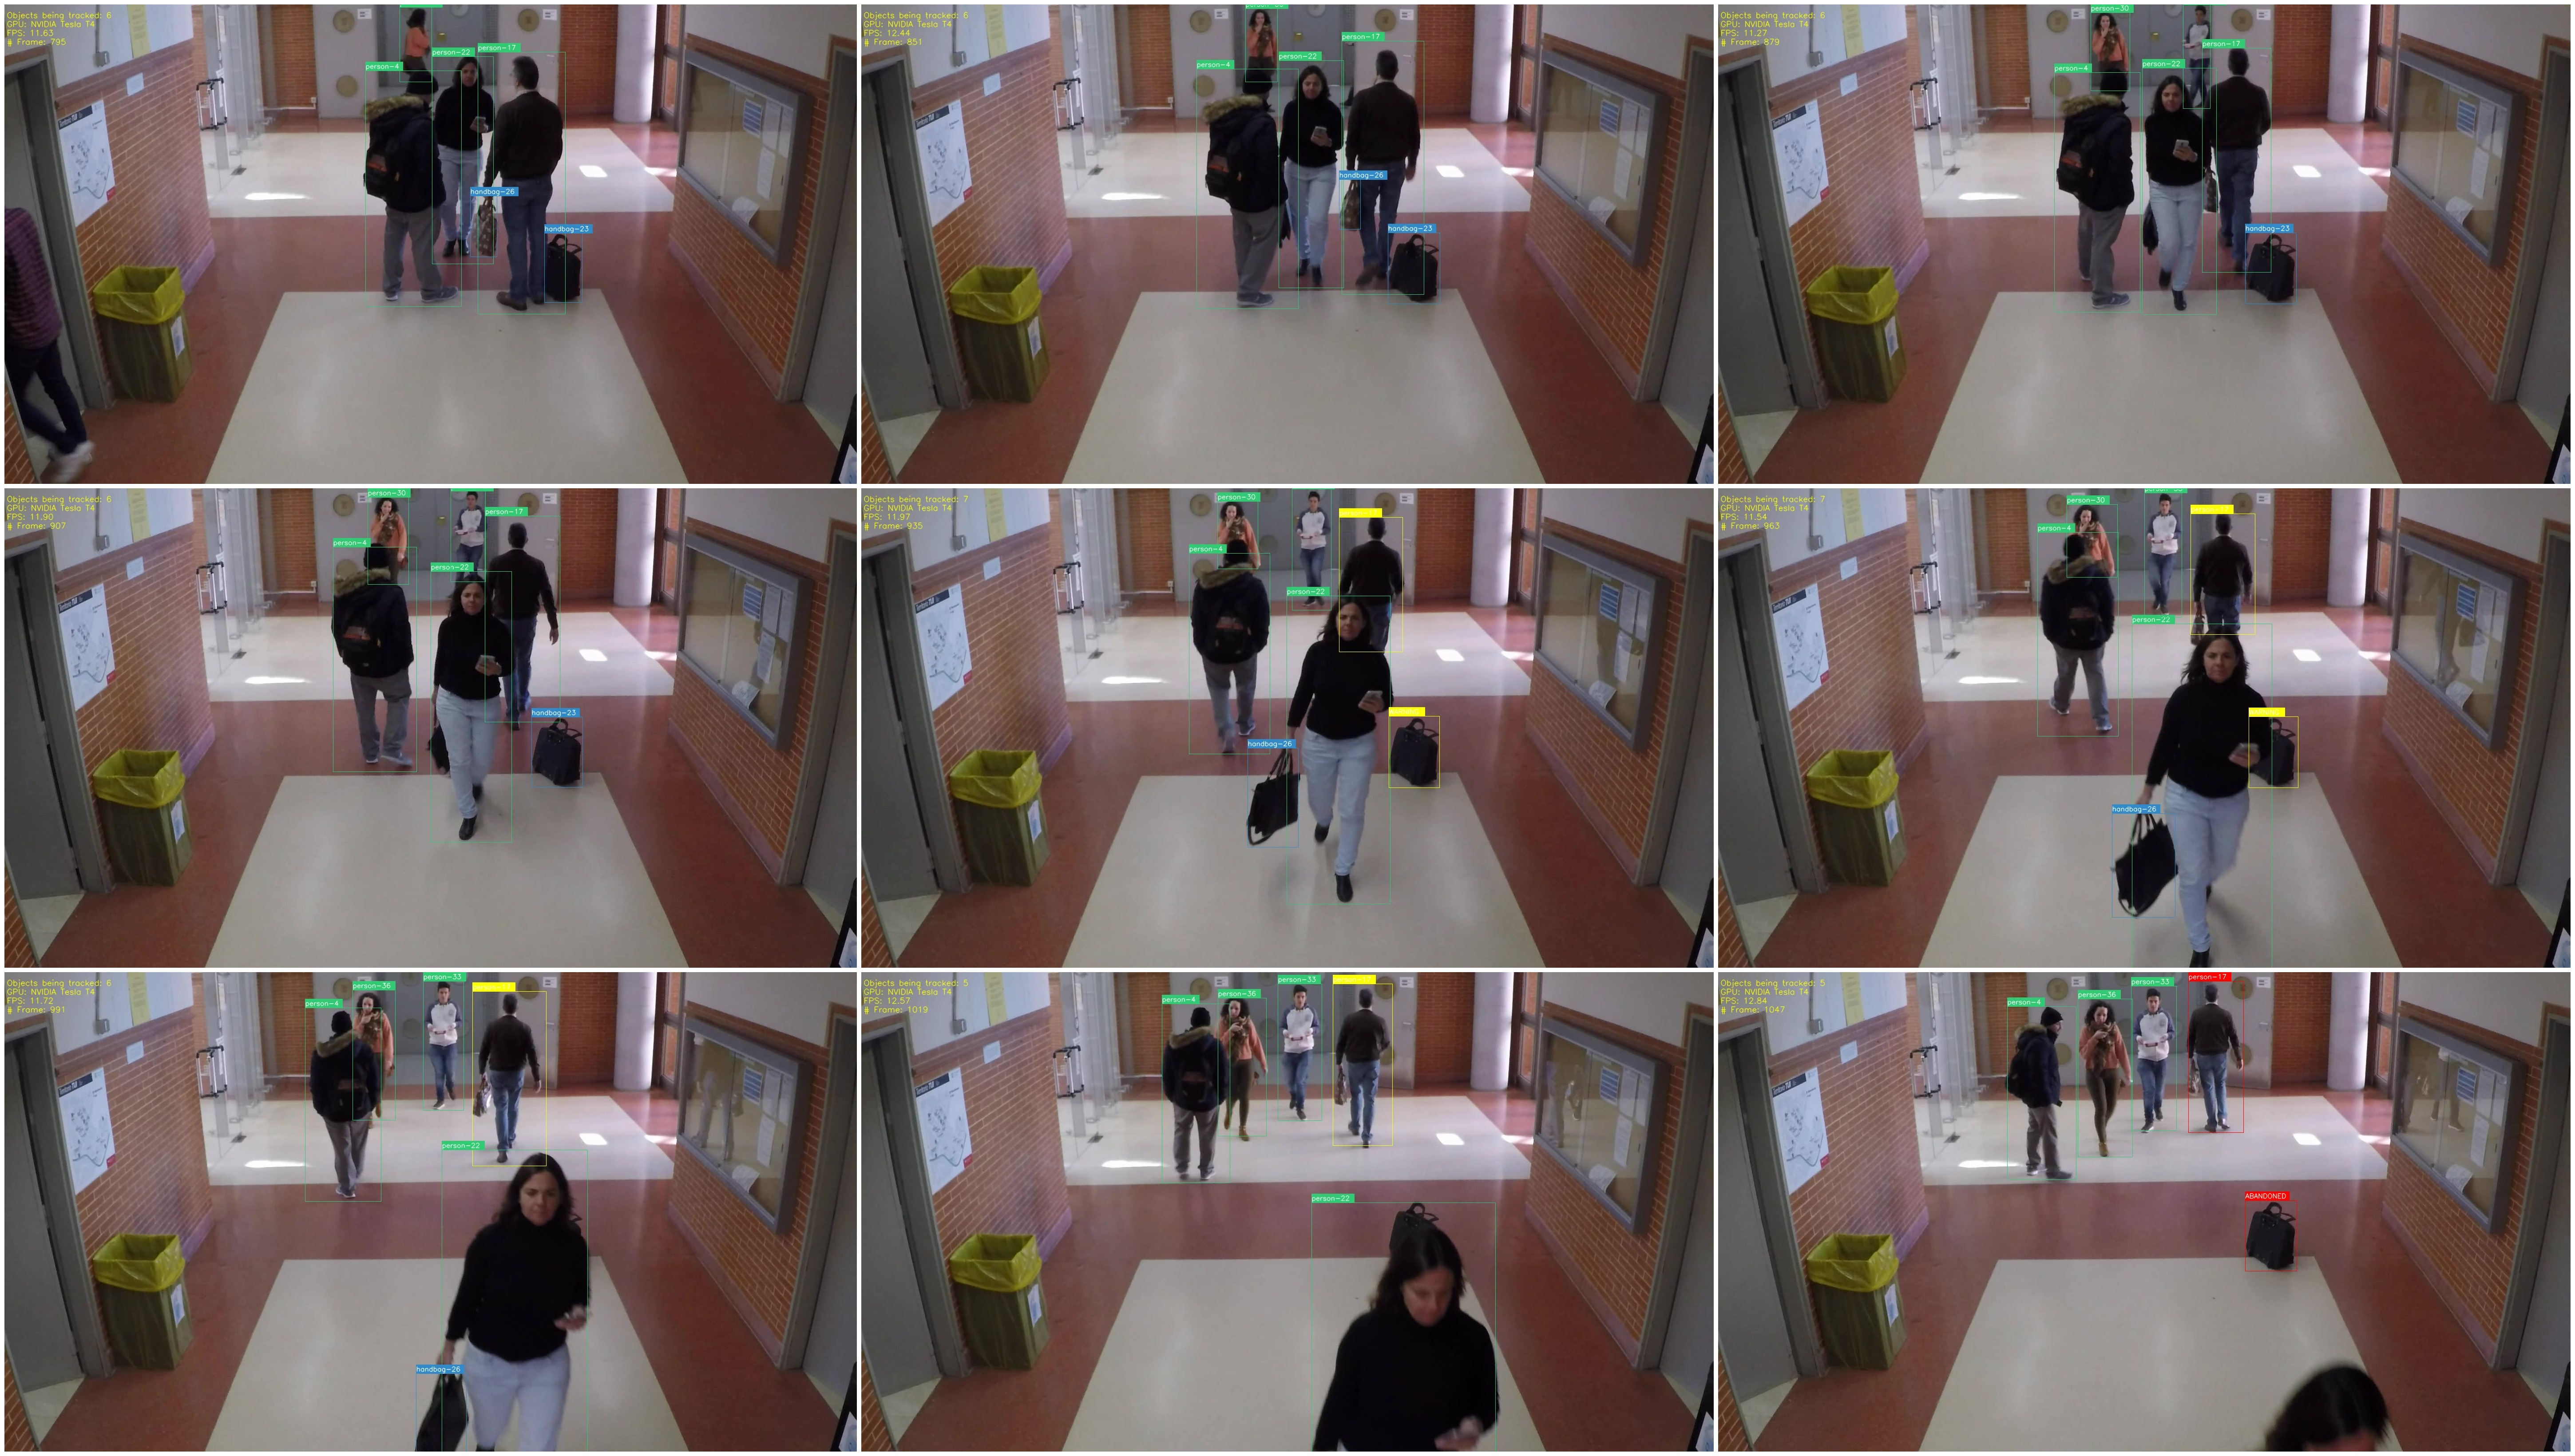
\includegraphics[width=0.9\textwidth]{Images/resultados/evaluacion-algoritmos/1.png}
\caption{\label{fig:abandono-uah1}Bolsa de mano abandonada en el pasillo de cafetería de la EPS (1)}
\end{figure}

\end{frame}

%%%%%%%%%%%%%%%%%%%%%%%%%%%%%%%%%%%%%%%%%%%%%%%%%%%%%%%%%%%%%%%%%

\begin{frame}{Resultados}{Resultados detección objetos abandonados}

\begin{figure}[ht]
\centering
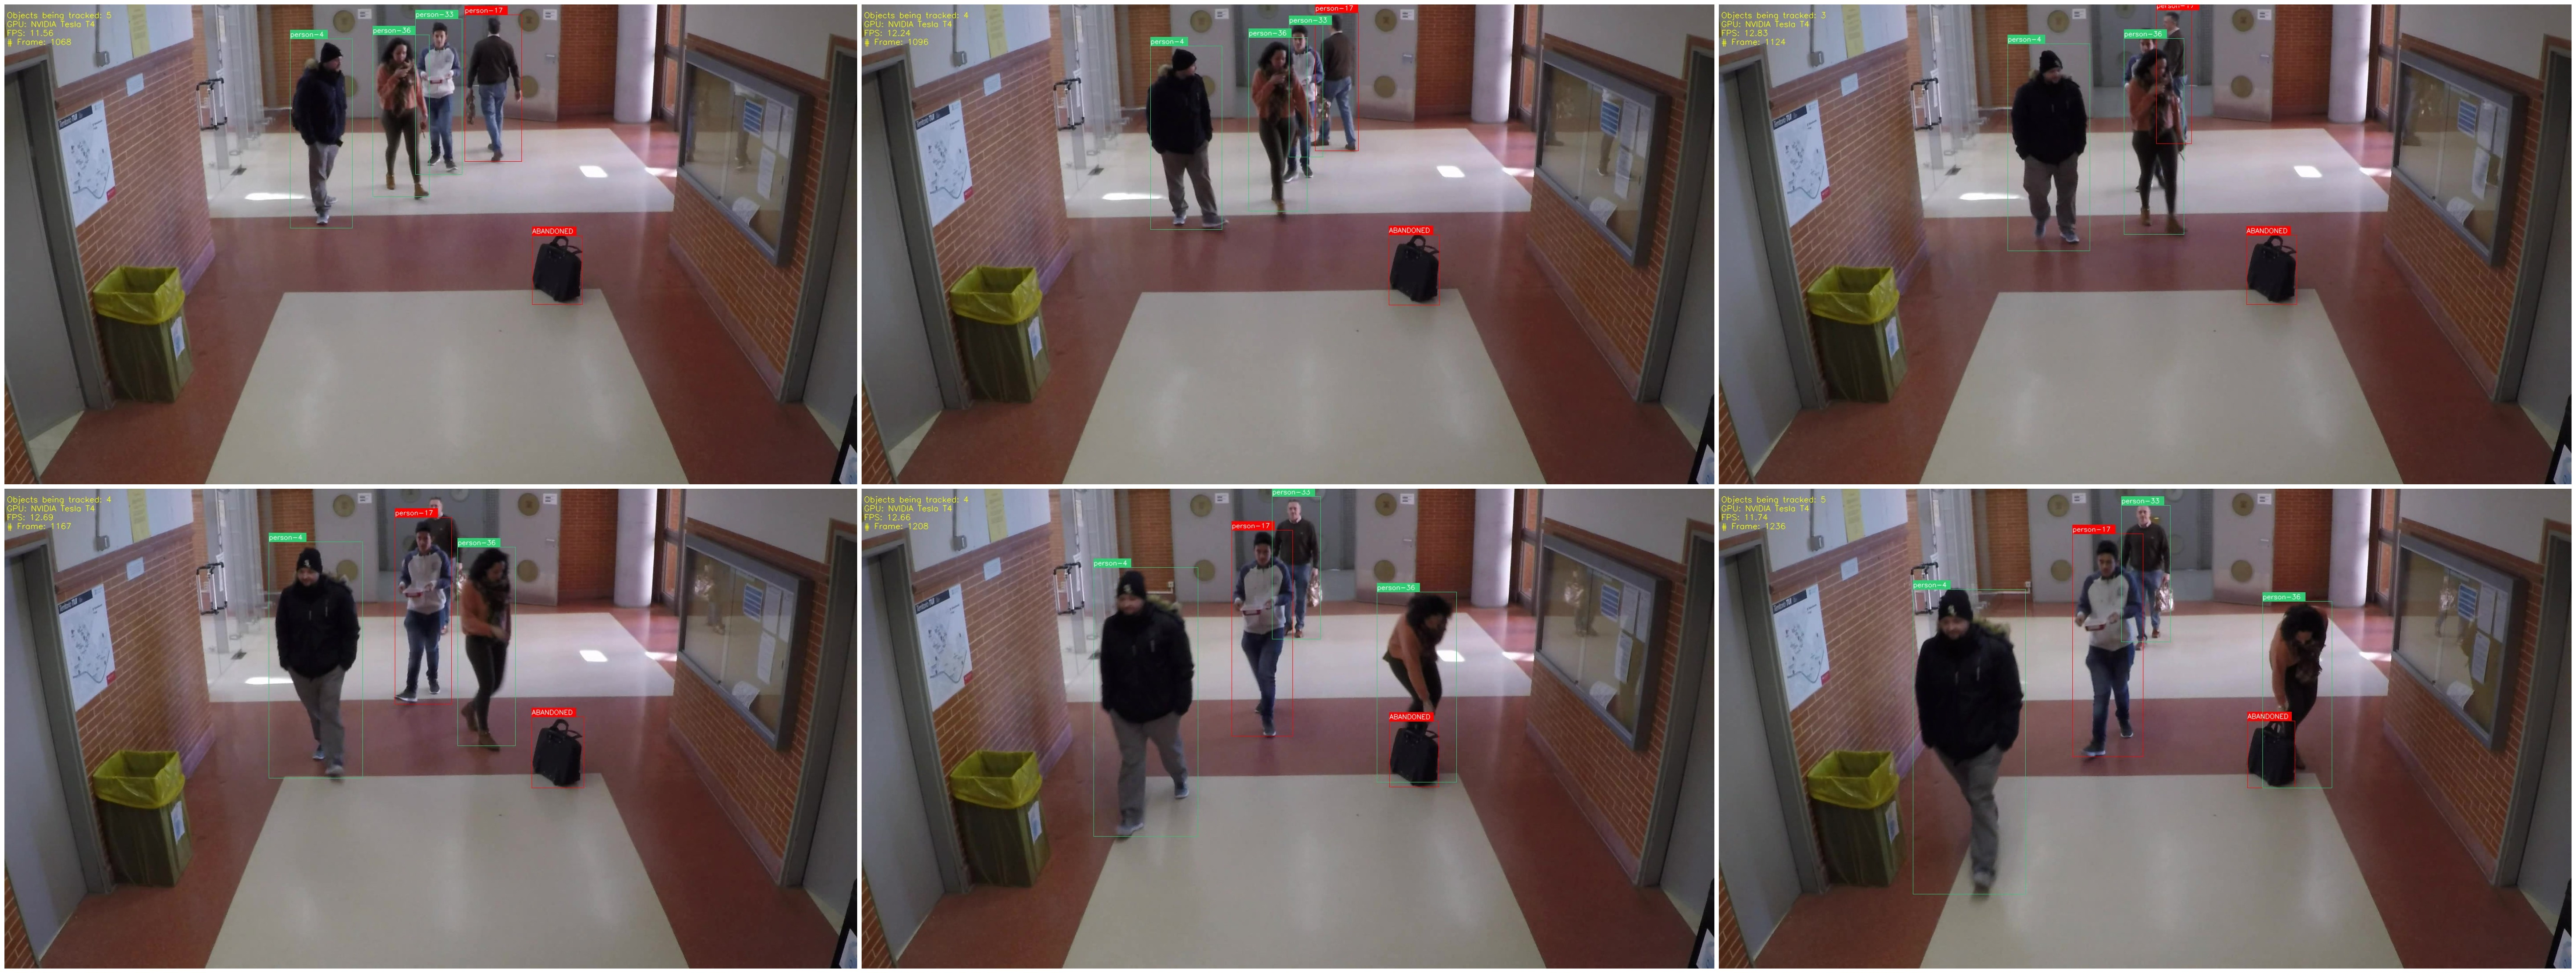
\includegraphics[width=1\textwidth]{Images/resultados/evaluacion-algoritmos/2.png}
\caption{\label{fig:abandono-uah2}Bolsa de mano abandonada en el pasillo de cafetería de la EPS (2)}
\end{figure}

\end{frame}